% ------------------------------------------------------------------------
% -*-TeX-*- -*-Hard-*- Smart Wrapping
% ------------------------------------------------------------------------

%REF_1 - J.A. Hartigan (1975). Clustering algorithms. John Wiley & Sons, Inc.

%REF_2 - Joblove and Greenberg’s (1978) HSL and HSV

%REF_3 - Charnes, A.; Frome, E. L.; Yu, P. L. (1976). "The Equivalence of Generalized Least Squares and Maximum Likelihood Estimates in the Exponential Family". Journal of the American Statistical Association. 71 (353): 169–171.

\def\baselinestretch{1}

\chapter{Proposed Approach 1: Using a Counting-by-Regression Method}

\def\baselinestretch{1.66}


%%% ----------------------------------------------------------------------

% intro text here
In this dissertation, two methods for counting wheat grains in images are proposed. This chapter presents the first method which takes a counting-by-regression approach. The high-level idea of this method is extremely simple: given $N$ training images with their grain counts provided, the goal was to recover a grain density function $F$ as a real function of pixels in the images. The grain density function learns the relationship between the density of spikelets in areas of the image and provides a mapping between said density and the number of grains in the image. New images could then be provided as input to $F$ and an estimate of the number of grains in the provided image returned as output. The grain density function (which serves as the predictive model) is built by constructing a regression model with the textural features computed from the GLCMs of the images in the dataset. The first step in this approach is the textural feature extraction from the images and the next step involves constructing the regression model. This chapter describes each step in the process.

\bigskip

%%% ----------------------------------------------------------------------
\goodbreak
\section{Textural Feature Extraction}
For the system proposed by this approach, all images dealt involved are dealt with as a representation of their textural features as opposed to the actual images themselves. Textures are complex visual patterns that have characteristics such as brightness, colour and contrast. Because of this, texture is easily perceived by humans and is believed to be a rich source of visual information. Because it is a rich source of visual information, it can be used as a metric for similarity between images as well as for characterizing images. 
\begin{figure}[ht!]
\centering
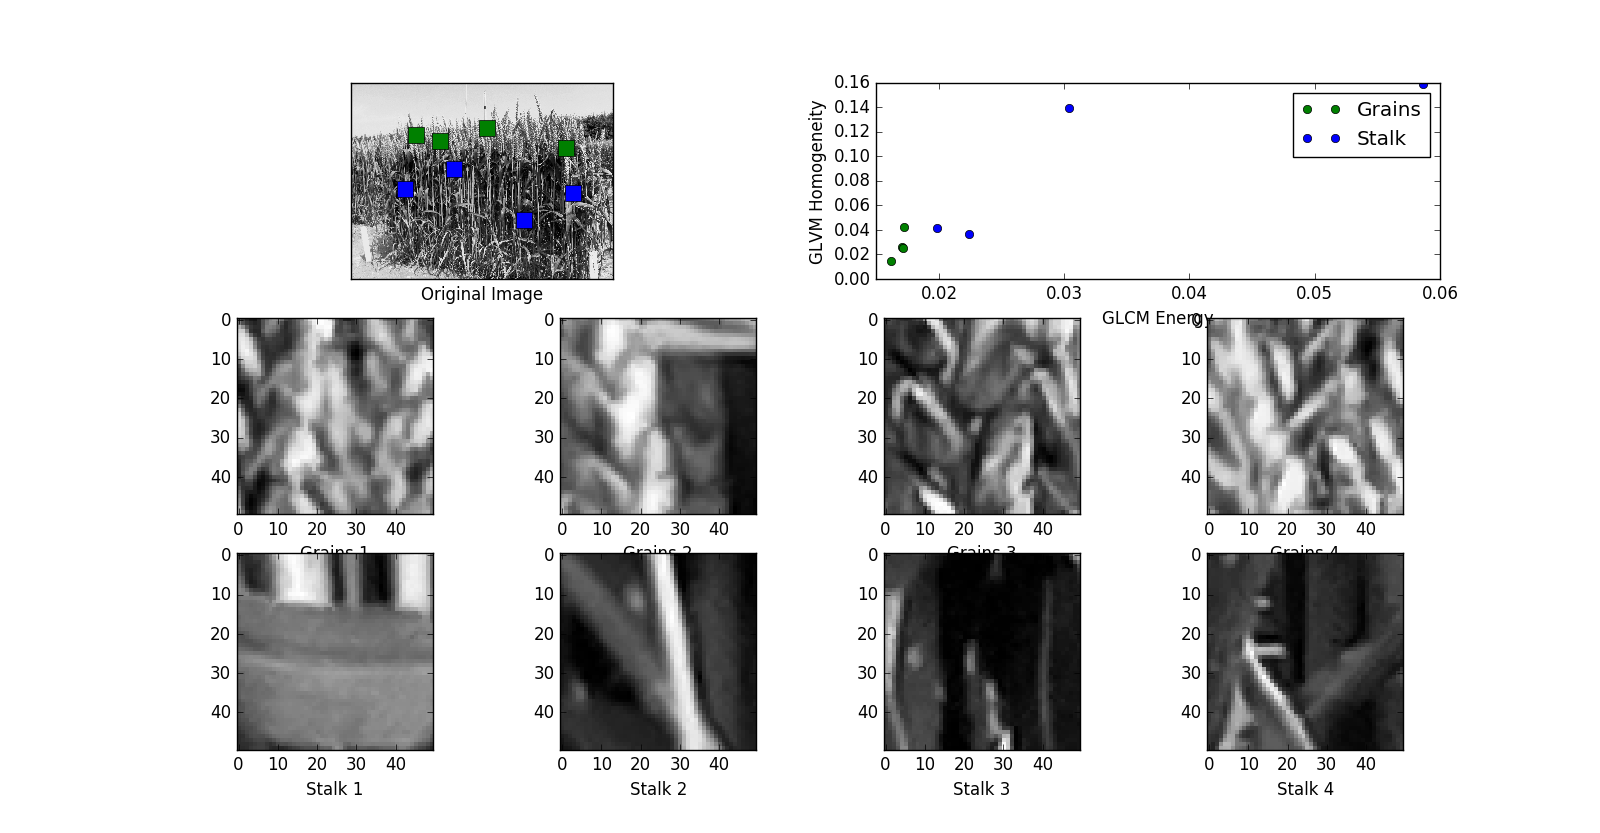
\includegraphics[scale=0.3]{glcm_1}
\caption{Plot of GLCM descriptors demonstrating their discriminative power}
\label{fig1}
\end{figure}
This approach makes use of \textit{Gray Level Co-occurrence Matrix} (GLCM) texture analysis. GLCM texture analysis was chosen as descriptors computed from the GLCM are quite discriminative. FIG\_ shows a two-dimensional plot of the GLCM features extracted from wheat grain images and wheat stalk images. It can be seen that GLCM descriptors are able to adequately discriminate between grain regions and stalk regions.\\ \\
%
For each image involved with the system in this approach, its GLCM is computed. In particular, the GLCM descriptors used to construct the feature vectors are \textit{energy (\textbf{ASM})}, \textit{contrast (\textbf{CON})}, \textit{homogeneity (\textbf{HOM})} and \textit{correlation (\textbf{CORR})}. Each of these descriptors is computed for an image for when the angle between neighbouring pixels $\theta = 0\circ$, $\theta = 45\circ$, $\theta = 90\circ$ and $\theta = 135\circ$ and the distance between neighbouring pixels, $d = 0$ to build a 16-dimension feature vector describing the image.

\bigskip
%%% ----------------------------------------------------------------------

%%% ----------------------------------------------------------------------
\goodbreak
\section{Building the Model: Linear Regression Analysis for Count Estimation}
The prediction model is developed by performing linear regression analysis on the set of extracted texture-based features. The model learns the relationship between the textural features of the image and the number of grains in the image. Regression analysis is a classic statistical method, and its basic idea is that given some value $y$ and another value $x$, which is a property of $y$, a function $y = f(x)$ is derived. This function $f$ can then be used to determine the value of $y\prime$ given $x\prime$, where $x\prime$ is a newly encountered value of $x$ and $y\prime$ is its corresponding value of $y$.\\ \\
The proposed framework makes use of a linear regression model with the count as the dependent variable and for each of the 4 texture descriptors in the 16-dimension feature vector, selects the most important values as independent variables. Recall that for each descriptor (\textit{energy}, \textit{contrast}, \textit{homogeneity} and \textit{correlation}), the value of the descriptor is computed in 4 different spatial arrangements $(d,\theta)$. This gives the values $ASM_{00}$, $ASM_{01}$, $ASM_{11}$, $ASM_{10}$, $CON_{00}$, $CON_{01}$, $CON_{11}$, $CON_{10}$, $HOM_{00}$, $HOM_{01}$, $HOM_{11}$, $HOM_{10}$, $CORR_{00}$, $CORR_{01}$, $CORR_{11}$ and $CORR_{10}$. Before building the regression model, Principal Component Analysis (PCA) is applied to the four values for the arrangement of each descriptor to yield one representative value for each texture descriptor giving $ASM\text{'}$, $CON\text{'}$, $HOM\text{'}$ and $CORR\text{'}$. The linear least squares method is used to compute the regression equation, ie. the model. (REF\_3). The linear regression model is of the form:
\begin{equation}
y = \alpha ASM\text{'} + \beta CON\text{'} + \gamma HOM\text{'} +\delta CORR\text{'}
\end{equation}

where $\alpha$, $\beta$, $\gamma$ and $\delta$ are constants calculated by performing a linear regression analysis on the set of training feature vectors and y is the count of grains in the image. Linear regression is used because it does not seem like too much of a stretch to assume that the relationship between the density of grains in an image is directly proportional to the number of grains in the image.
\bigskip
%%% ----------------------------------------------------------------------

%%% ----------------------------------------------------------------------
\goodbreak
\section{Counting With the Regression Model}
The only thing needed to count grains in images with this method is the regression equation, more specifically, the estimated coefficients and potentially, the intercepts. This means that the model can be represented in simple terms that are easily readable, understandable and accessible to humans (that aren't necessarily familiar with statistical modelling). It also means that the model can easily be stored and shared once it is computed with little or no cost.\\ \\
%
Given a query image whose grain count is desired, the query image is first converted to a textural representation by extracting its GLCM texture features and forming the feature vector as described in the previous section. PCA is applied to each group of the four descriptors in the 16-element vector to yield one representative value for each texture descriptor giving $ASM\text{'}$, $CON\text{'}$, $HOM\text{'}$ and $CORR\text{'}$. To obtain the grain count, the calculated coefficients (and potentially, intercepts) are substituted into FIG\_ with the descriptor values. The solution of the equation is the estimate of the number of grains in the image. 
\bigskip
%%% ----------------------------------------------------------------------


%%%%%%% APPROACH 2 %%%%%%%%%%%%

\def\baselinestretch{1}

\chapter{Proposed Approach 2: Using a Counting-by-Detection Method}
\def\baselinestretch{1.66}


%%% ----------------------------------------------------------------------

% intro text here
The proposed solution takes a counting-by-detection approach to solving the problem. It makes use of both image analysis and computer vision techniques and machine learning techniques. The detection of grains to be counted is carried out in a supervised learning manner and the image is manipulated using computer vision techniques. The system aims to first detect all instances of grains in a given image, then compute the count as the number of instances detected. FIG\_ illustrates the design of the system and its various components. The system first pre-processes images, extracting the regions of interest, then breaks the image into  thousands of sub-images. The sub-images are then passed to a classifier which has been trained initially and thus predicts whether a sub-image contains a grain or not. This chapter proposes a solution to the problem of counting the number of grains in an image. The proposed system is broken down into stages and each stage is described in this chapter.

\smallskip

\begin{figure}[ht!]
\centering
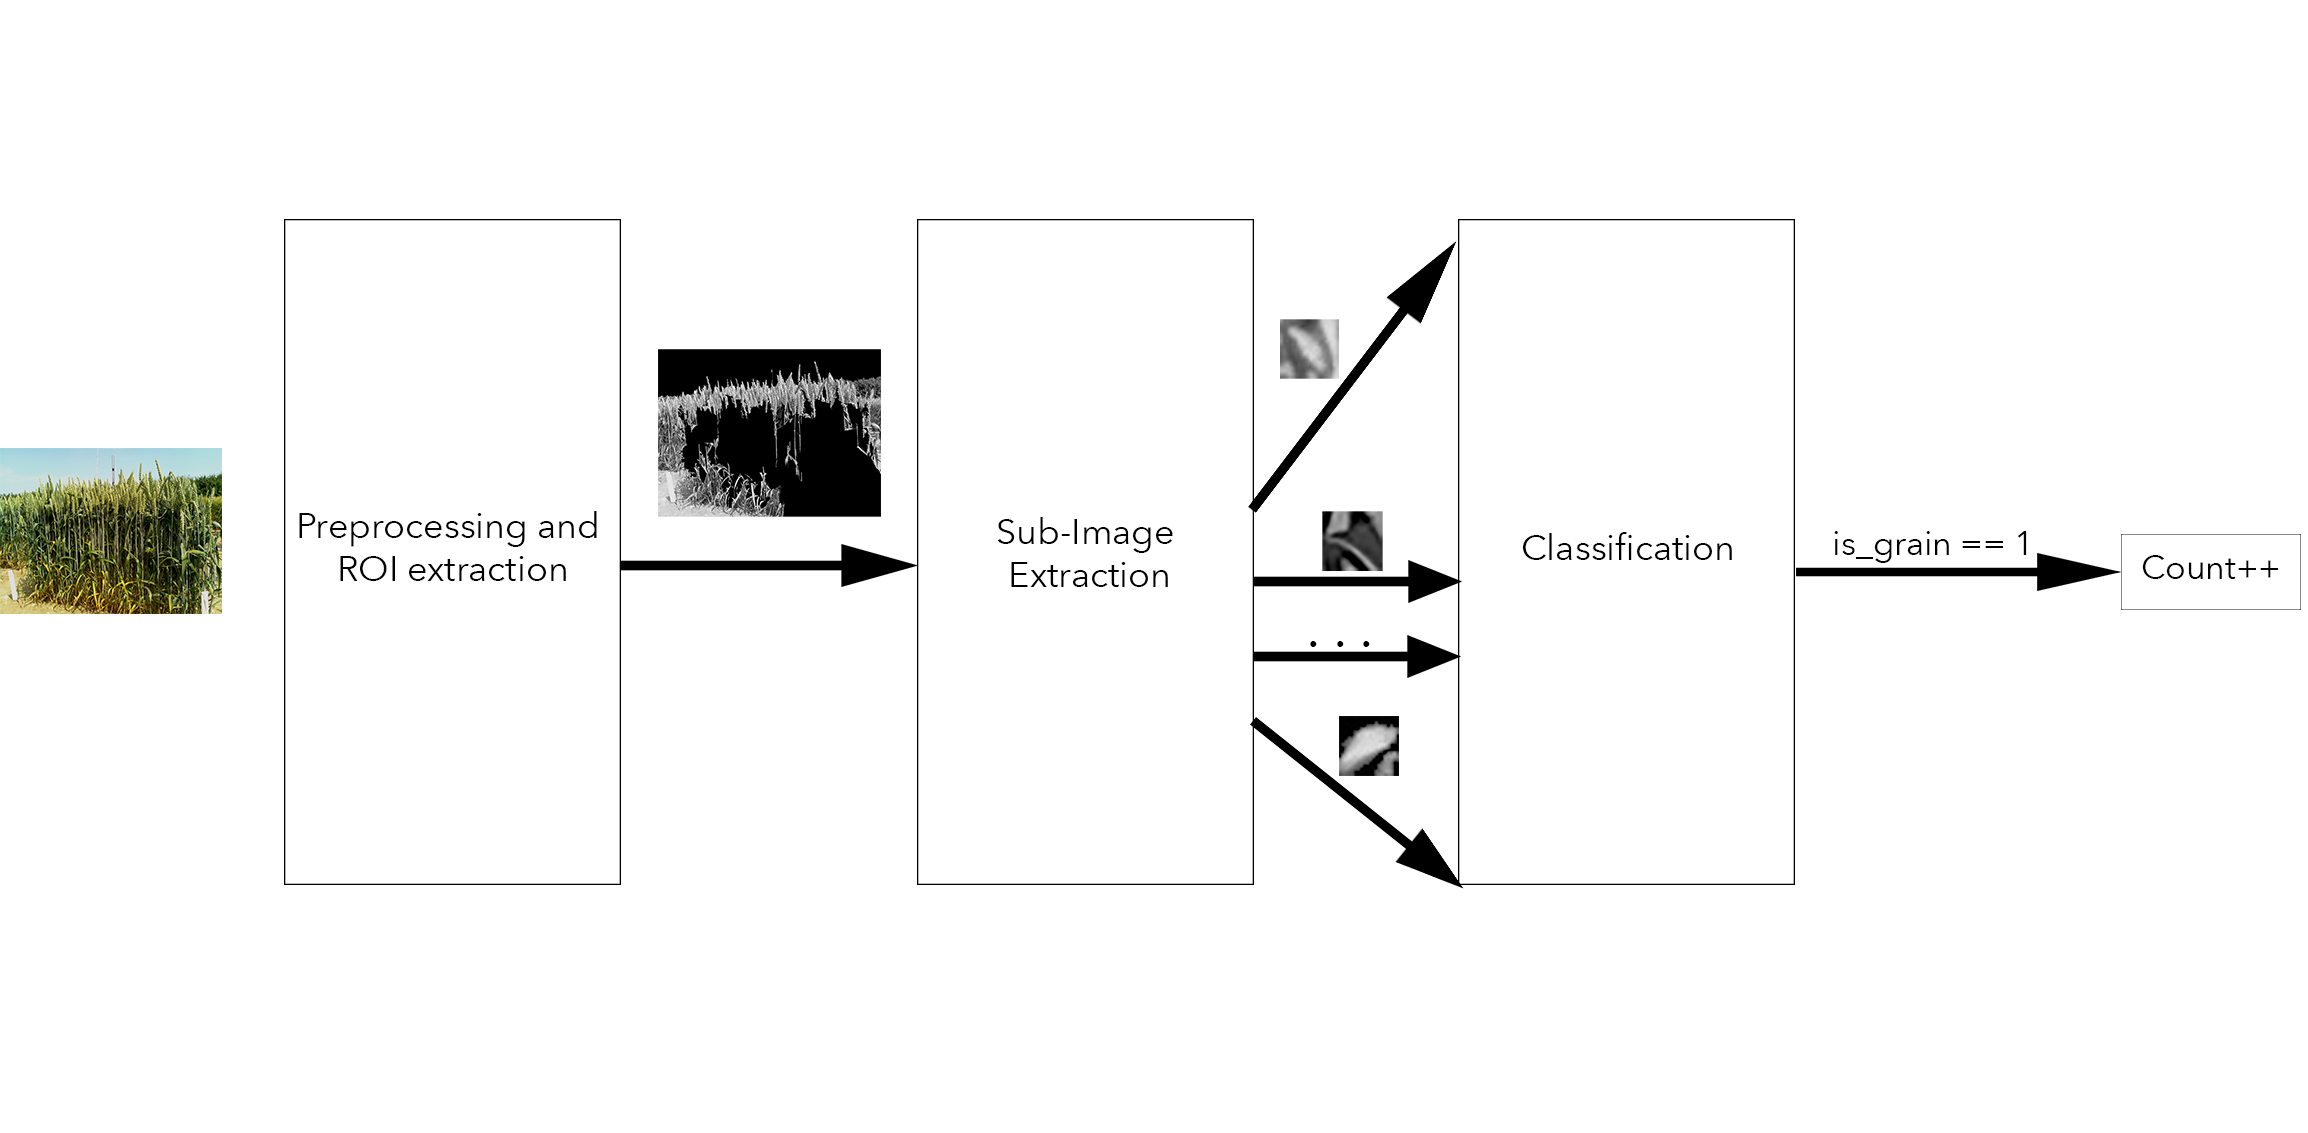
\includegraphics[scale=.4]{Images/design_pipeline}
\caption{Placeholder for diagram showing system overview and components}
\label{fig1}
\end{figure}

\smallskip

%%% ----------------------------------------------------------------------
\goodbreak
\section{Grain Counting Pipeline}
\subsection{Image Pre-processing}
The first step in the grain counting process is to identify and remove all parts of the given images that do not contain grains. The aim of this stage is to reduce the problem space by extracting only the regions of the images that we are concerned with - that is, the spikelets and grains. Region of Interest (ROI) extraction also makes the grain detection and counting process accurate. It removes sky, ground, leaves, and background regions from the image. Otherwise, parts of these regions could be wrongly detected as grains and counted.\\ \\
%
ROI extraction is achieved using \textit{segmentation-based object categorization}. This process applies spectral clustering to an image in order to partition the image into distinct regions, known as clusters, based on their colour. The pixels in a cluster are similar to each other in colour but different from pixels in other clusters. In this project, the \textit{\textbf{k-Means Clustering}}(REF\_1) algorithm is used to cluster the pixels. Given an image of $n$ pixels ($x_1, x_2, ..., x_n$) in the HSV space (REF\_2) where each element $x_i$ is a vector made up of that pixels hue, saturation and value, we partition the $n$ pixels into $k$ clusters, $C = \{C_1, C_2, ..., C_k\}$ in order to minimize the distance between every pixel and the mean pixel in each cluster. Mathematically, the spectral clustering via kmeans can be denoted as:

\begin{equation}
argmin \sum_{i=1}^{k}\sum_{x\in C_i} ||x - \mu_i||^2
\end{equation}

where $\mu_i$ is the mean HSV pixel vector in cluster $i$\\ \\
%
FIG\_ shows an illustration of the ROI process. The original image has spectral clustering applied to it as described above (with $k = 5$), and the result of this is shown in FIG\_(a). Each cluster is shown with a different colour overlayed over it. From this image, we can select the clusters which contain relevant information (grains) and do away with other clusters. FIG\_(b) illustrates this as it shows the resulting image after the red, green and purple clusters are removed. The resulting ROI image contains still contains all of the useful information (ie. grains) but only little else.
\begin{figure}[ht!]
%\centering
\begin{subfigure}{.5\textwidth}
%  \centering
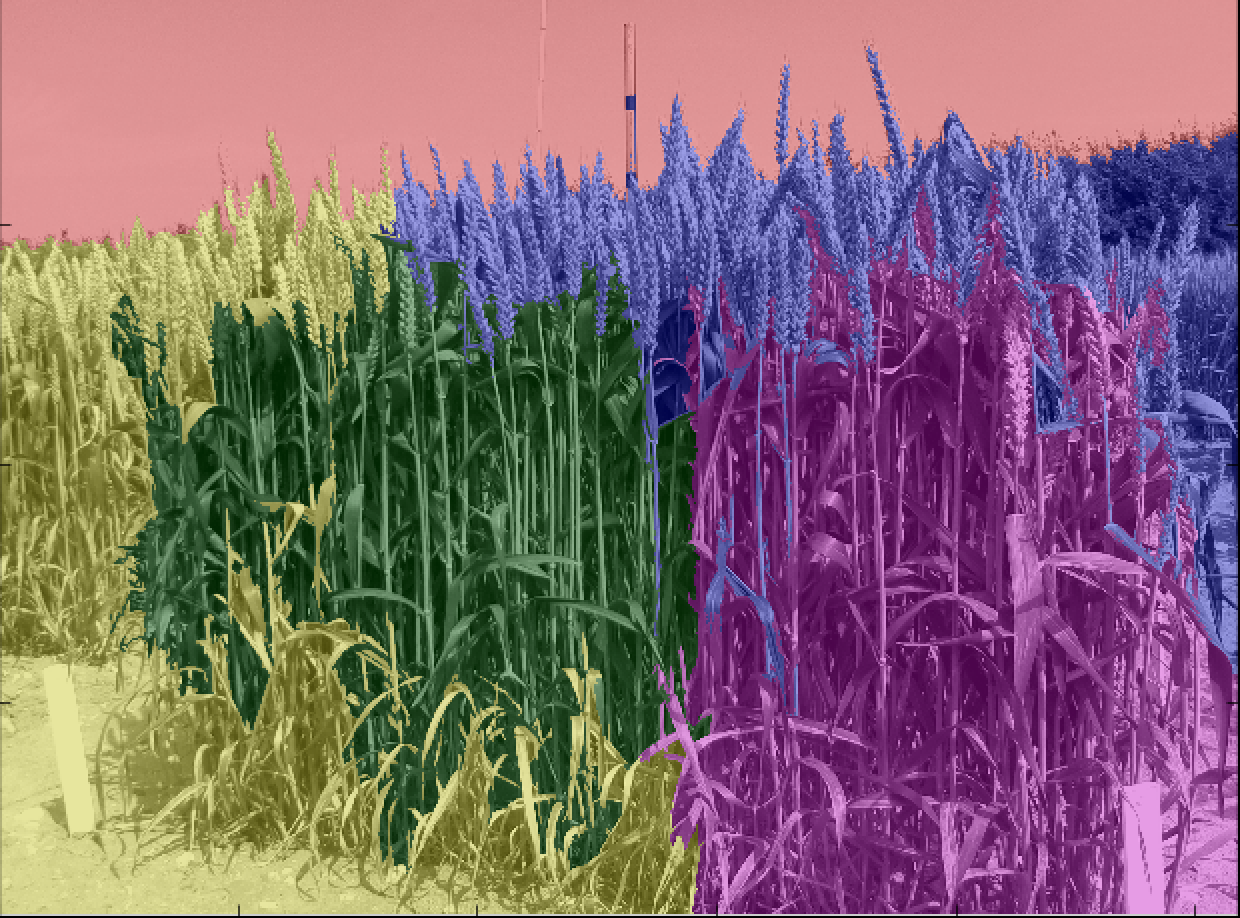
\includegraphics[width=.9\linewidth,height=.7\linewidth,keepaspectratio]{clusters.png}
  \caption{Image showing cluster memberships}
  \label{fig:sub1}
\end{subfigure}%
\begin{subfigure}{.5\textwidth}
%  \centering
 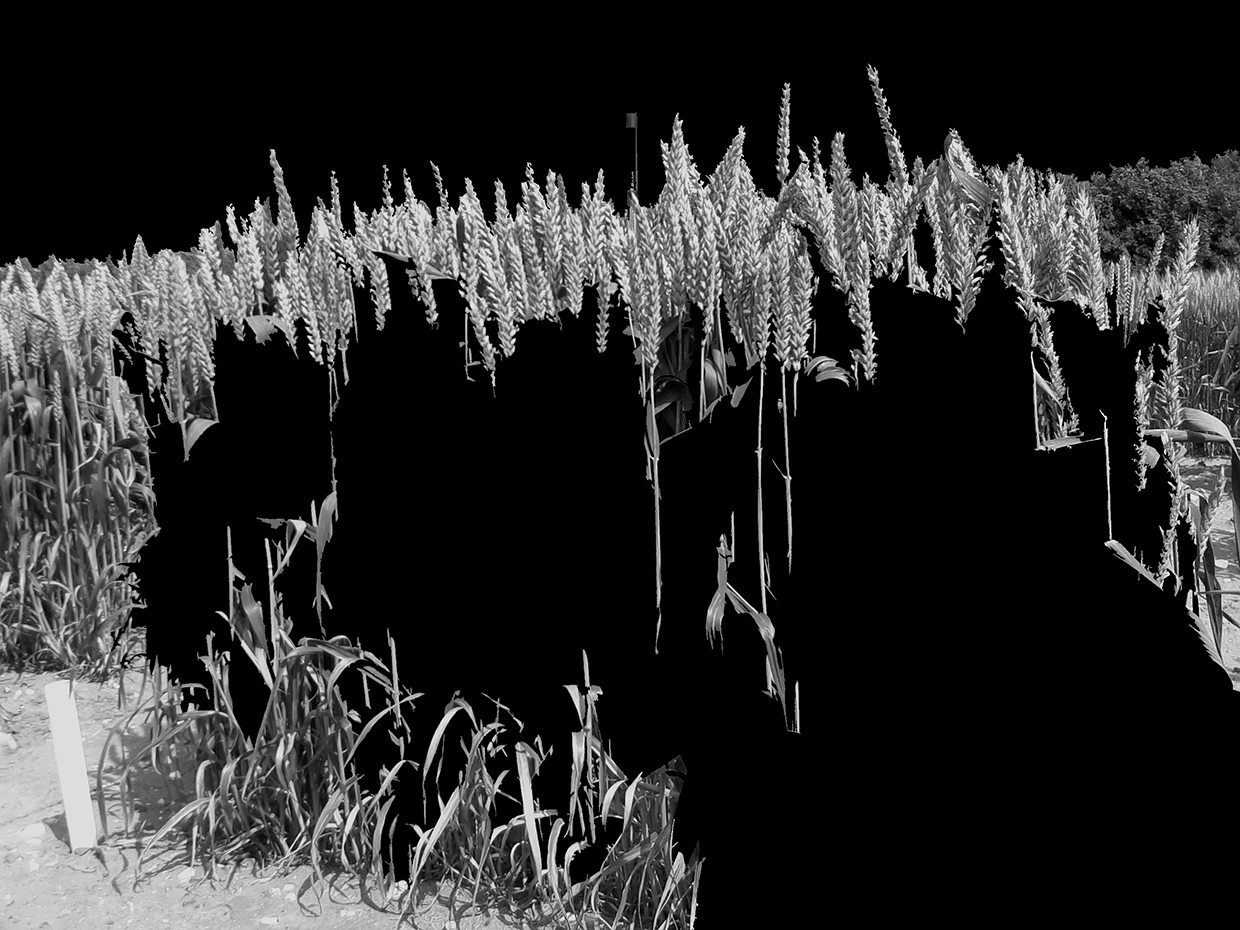
\includegraphics[width=.9\linewidth,height=.7\linewidth,keepaspectratio]{roi.png}
  \caption{ROI image with useful clusters extracted}
  \label{fig:sub2}
\end{subfigure}
\caption{ROI extraction using spectral clustering}
\label{fig:test}
\end{figure}

\subsection{Sub-image Extraction}
The next step in the grain counting process is to break the extracted ROI image into tiny blocks. These blocks might contain grains or they might contain stalks and leaves that were overlooked in the ROI extraction process. A conceptual summary of the proposed system is that it counts which of these blocks contains a grain, thereby giving a grain count for the whole image. However, it is important to also note that one block might contain more than one grain or even only a portion of a grain. So if the conceptual description is applied, the result would not be very accurate. Strictly speaking, the system only yields an estimate of the grain count. To make this estimate as accurate as possible, the division of the image into blocks has to be done as precisely as possible, with blocks containing grains having either just one grain or a large portion of a grain in them.\\ \\
%
The blocks are extracted using a kernel convolution approach. The convolution matrix (or kernel) is an $M$-by-$N$ matrix containing all $1$s. First the image is transformed to greyscale to simplify the convolution process. Each time the kernel is applied, the result of the convolution is stored in a list. Edges are handled using a ``cropping'' approach. That is, if the kernel cannot completely be placed at an edge, that edge is simply ignored.
\begin{figure}[ht!]
\centering
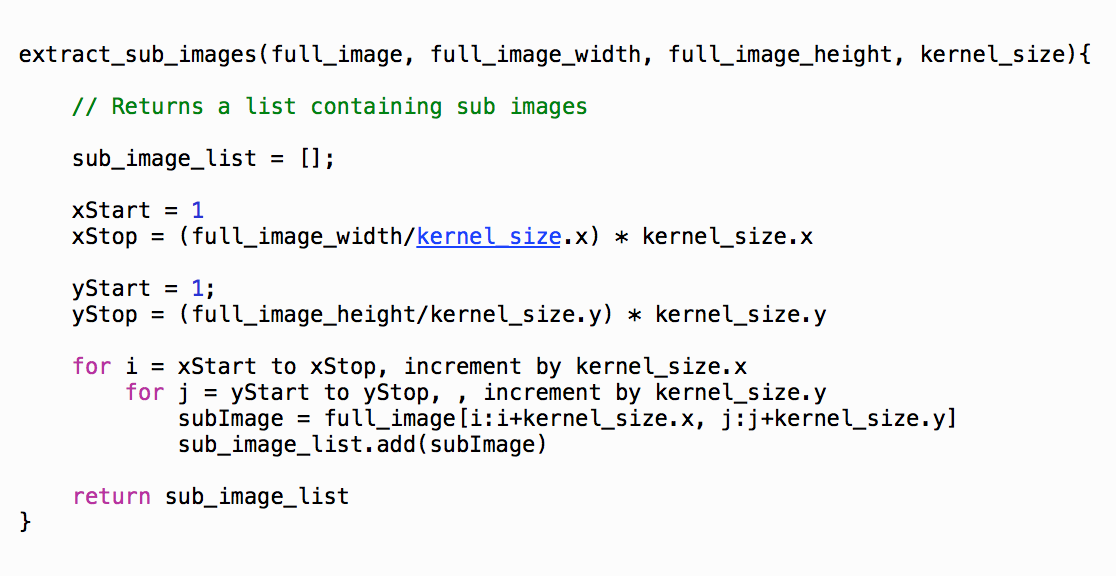
\includegraphics[scale=0.6]{kernel}
\caption{Pseudocode of sub-image extraction using kernel method}
\label{fig1}
\end{figure}
In our implementation, we use a kernel of size $20$-by-$20$ giving square sub-images of length $20$. This value is ideal because it is large enough to contain one grain. Due to visual perspective issues, grains closer to the background appear smaller. A $20$-by-$20$ kernel is still small enough to contain only one or one and a bit more of a grain scaled down. Also, with a kernel of this size, the cropping edge handling approach is of no negative consequence as it highly unlikely that more than a minuscule number of grains will be in the remainder of the edge (which would be less than $20$ pixels wide).

\subsection{Classification}
This is the main step in the grain counting process. Here, the sub-images extracted from the previous step are classified as either containing a grain or not. In particular, a \textit{\textbf{Multi-Layer Perceptron (MLP)}} neural network is used for the classification. The neural network does not deal directly with the images as a whole, but rather with sub-images. Recall that our dataset contains only $13$ images which would not be anywhere near sufficient to properly train the neural network. However, because the neural network deals with sub-images, it can be trained using just one of the images in the dataset. When this one image is selected, it can then be broken down into its sub-images of size $20$-by-$20$. Each image yields $5000$ sub-images on average. This is more than sufficient for training the neural network. Unfortunately, the generated sub-images will still need to be labeled in order to be used for training the neural network. This would be a very time consuming and labour-intensive task. Because of this, only $350$ sub-images were hand selected and labeled. The neural network is then trained on these sub-images. When selecting sub-images to be used for training the neural network, care was taken to keep the training data balanced. That is, the numbers of grain sub-images and non-grain sub-images were fairly close. No one class dominated the selected sample.\\ \\
%
It is worth noting that the whole sub-images are not passed into the neural network. Instead, discriminative features are extracted from the sub-images to form feature vectors. We make use of textural features based on the textures of the sub-images. Generally speaking, textures are complex visual patterns that have characteristics such as brightness, colour and contrast. Because of this, texture is easily perceived by humans and is believed to be a rich source of
visual information. For each sub-image, the \textit{Gray Level Co-occurrence Matrix (GLCM)} is computed. From the GLCM, we then compute the following texture descriptors - \textit{energy}, \textit{homogeneity}, \textit{correlation} and \textit{dissimilarity}. Each of these descriptors is computed for when $\theta = 0^\circ, \theta = 45^\circ, \theta = 90^\circ$ and $\theta = 135^\circ$ and the distance, $d = 0$ to build a 16-dimension feature vector describing the sub-image. This means that 16-element vectors are passed through the neural network, as opposed to $20$-by-$20$ matrices (400-element vectors). This saves memory and also allows the neural network to work faster as well. FIG\_ shows GLCM descriptors extracted from different parts of a wheat image and plotted against each other. From the figure, it can be seen that GLCM descriptors are able to adequately discriminate between grain regions and stalk regions. By using GLCM feature vectors instead of raw image data, we can boost the discriminative power of the neural network and improve the accuracy of the detection system.

\subsection{Employing the System to Counting}
Once the neural network is built, it can then be used for the detection of grains. Given a query image, it is passed through the pipeline. First, the query image goes through pre-processing to have the ROI extracted from it. The query ROI image is then broken into query sub-images. Next is the detection stage - the neural network is applied to the query sub-images to determine whether a given sub-image contains a grain or not. The number of sub-images classified as containing grains by the neural network is then returned as an estimate of the number of grains in the image.
\bigskip

%%% ----------------------------------------------------------------------
\goodbreak




\bigskip

%%% ----------------------------------------------------------------------


